\section{Introduction}
\label{sec:introduction}

AI-generated updates can become persistent facts used for reporting, payment, scheduling, or later decisions. Admission must therefore establish which authority approved which value from which persisted proposal and record state.

Consider a record whose authoritative quantity is 90. A recognizer proposes 100, but a reviewer authorizes 101; an unchanged batch-code field should retain its earlier source. Accepting a machine proposal of 101 would produce the same final value with different attribution. Rewriting the candidate would falsely attribute the correction to the model, while dropping the unchanged field's source would preserve values but lose lineage. Admission must retain the predecessor 90, the proposal $x_c=100$, and the authorized value $x_a=101$, allowing
\begin{equation}
x_c\neq x_a
\label{eq:intro-correction}
\end{equation}
with both value roles and the complete successor's sources intact.

The target systems permit human correction of AI-generated field candidates, persist accepted updates as operational facts, and require later reconstruction of authorization and origin. Existing activation, governed-memory, and transaction mechanisms provide adjacent foundations: Continuity Kernel separates candidates from atomic activation; LatticeMind handles claim selection and supersession; authority-collapse work studies lost source constraints; MutMem binds authorized changes to predecessor history; and MemTxn supports source-grounded updates and recovery \citep{he2026continuity,zhou2026latticemind,zhan2026authoritycollapse,saidi2026mutmem,cui2026memtxn}. We specialize this problem to the following correction-aware, field-level relation:
\begin{equation}
\begin{aligned}
\textit{exact candidate}
&\rightarrow\textit{candidate-bound human authorization}\\
&\rightarrow\textit{explicit authorized value}
\rightarrow\textit{complete successor}\\
&\rightarrow\textit{total field-source attribution}.
\end{aligned}
\label{eq:admission-chain}
\end{equation}
The candidate remains historical evidence; human authorization supplies value authority; a trusted transaction constructs the successor. Ordinary transaction and logging facilities can implement this relation. The engineering increment is their joint, checkable binding of proposal identity, a possibly different authorized value, and exact changed/unchanged field sources.

We ask which observable distinctions preserve that relation against candidate substitution, correction erasure, stale replay, fragmented successors, and source ambiguity. Under a declared failure and observation model, paired histories expose what becomes indistinguishable when each information class is omitted. We study the relation through the Python/SQLite reference realization \system{}:
\begin{enumerate}[label=\textbf{C\arabic*:},leftmargin=*]
\item \textbf{Correction-aware admission contract.} Bind authorization to the exact candidate, keep proposed and authorized values separately attributable, and retain total field sources in one complete successor.
\item \textbf{Conditional failure distinguishability.} Five safe/unsafe history pairs establish class-wise irredundancy within the declared observation model, rather than a complete taxonomy of admission failures.
\item \textbf{Relational and transactional realization.} Connect the contract to bounded Alloy checks, a CAS-protected transaction, selected formal--concrete projections, and an executable fault catalogue.
\item \textbf{Cost and integration evidence.} Characterize frozen v8 persistence-equivalent admission and trace costs, and separate restricted-agent task outcomes from host-enforced authority checks across three qualified configurations.
\item \textbf{Standard-practice boundary.} Constructed transactional value-audit controls agree with candidate-bound admission on seven of eight single-history cases. Equal-valued candidate substitution separates them. Enriched review-context snapshots resolve differences they record, while exact candidate binding distinguishes persisted instances that remain equivalent under those snapshots.
\end{enumerate}

\paragraph{Illustrative workflow (a constructed example, not a deployment study)}
An operations team must be able to answer, months later, which persisted proposal a named reviewer actually inspected. Two retries of the same extraction produce candidates whose record, field, and authorized value are identical and whose creation timestamps and evidence locators differ. Under a value-level approval both candidates satisfy the recorded authorization, so an auditor reconstructing that review cannot tell which of the two it saw; under candidate-bound admission the authorization names one of them and the other is rejected. Which behaviour is required depends on the audit question. Where the question is only whether a value was approved, value-level approval is sufficient and the distinction adds nothing. It is needed where the question is which instance was reviewed, for attributing a decision to one specific artifact rather than transferring it silently between equal-valued instances. The present admission path records value-changing updates; a renewed review that leaves the value unchanged needs a separate review-event path.

Host authentication and review-channel integrity remain external assumptions: the contract records and rechecks authority, but it does not implement a complete access-control or anti-prompt-injection system.

The evaluation follows three levels: finite relational encodings (RQ1--RQ2), persisted implementation behavior and executable relation controls (RQ3--RQ5), and cost and agent integration (RQ6--RQ8). The relation controls test whether increasingly rich transactional audit state entails the candidate-level authorization relation, and identify the review-observation equivalence boundary at which exact persisted identity remains discriminating; the agent study supplies integration evidence. \Cref{fig:admission-workflow} shows the admission boundary; \cref{sec:related,sec:contract} position and define the relation.

% FIGURE SOURCE: scripts/build_flowcharts.py; vector redraw preserving the author-approved workflow semantics.
\begin{figure*}[t]
\centering
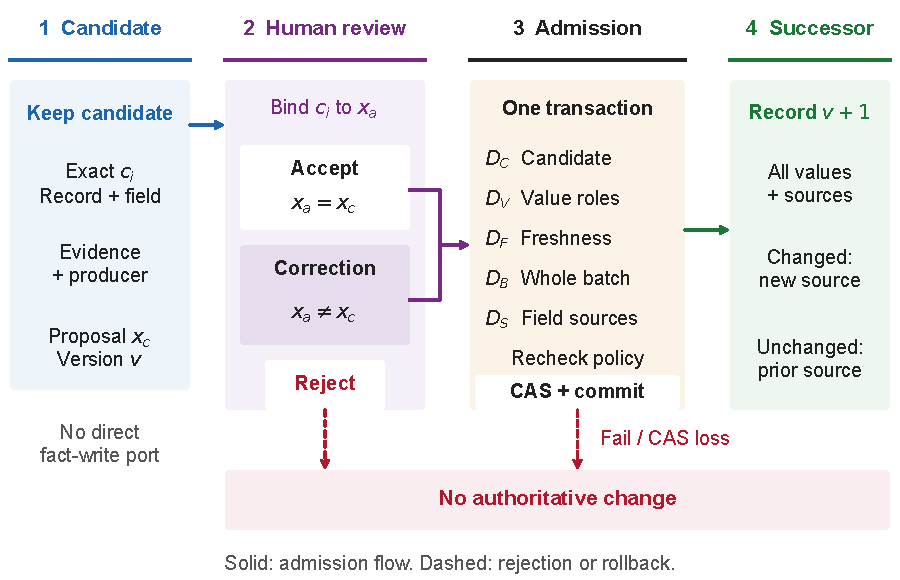
\includegraphics[width=0.96\textwidth]{figures/refined/figure-1-admission-workflow.pdf}
\caption{Correction-aware authoritative-state admission. Only candidate-bound Accept or Correction decisions proceed to transactional admission. The declared distinction checks, host-policy revalidation, and version compare-and-swap protect creation of a complete successor and total source map. Reject, failed validation, or a lost compare-and-swap leaves authoritative state unchanged. Authorization records responsibility, not factual truth. AI-assisted diagram scripting: OpenAI Codex (gpt-6-astra, OpenAI, September 2026 revision); deterministic vector rendering of the declared workflow.}
\label{fig:admission-workflow}
\end{figure*}
